\section{Recursos principals del bloc Memòries}

    \paragraph{}
    El bloc Memòries és relativament nou a l'API de FamilySearch i la documentació al respecte és pràcticament inexistent. Aquest bloc conté les memòries penjades al núvol pels usuaris i són relacionades amb les persones de l'arbre familiar.

    Recordem, que el concepte memòries ha estat descrit a la secció tres de la memòria, `L'organització Familysearch' i consisteixen principalment en contingut fotogràfic, històries, documents diversos i fitxers d'àudio.

    El recurs principal d'aquest bloc és el recurs Memòria, que conté tota la informació específica d'aquesta. Les memòries també contenen comentaris, en un estil molt similar a les discussions i també disposen de recursos intermedis per relacionar les memòries amb les persones a les quals fan referència. Com sempre, moltes d'aquestes connexions són implementades a través d'enllaços hypermedia.

    De moment, resulta necessari crear una instància del recurs Memòria per cada contingut que es vulgui pujar al sistema, però la possibilitat de suportar més d'un artefacte amb el mateix recurs memòria ha estat estudiat i en algun moment o altre serà implementat. Un exemple  de cas d'ús podria ser la necessitat de pujar les dues cares d'una fotografia.

    La imatge~\ref{img:memoriesBloc} ofereix un esquema de forma visual de com es relacionen els recursos vinculats al bloc Memòries.

    \begin{figure}[h]
        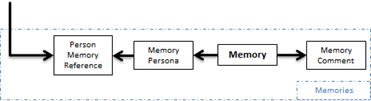
\includegraphics{05/06_memoriesCore}
        \centering
        \caption{El bloc de l'arbre familiar relatiu a les memòries}\label{img:memoriesBloc}
    \end{figure}

    Desgraciadament, la documentació referent a aquest apartat per part de FamilySearch és molt pobre i el contingut de cada un dels recursos ha estat creat per inferència mitjançant el collage de petites peces d'informació i les similituds que presentaven amb altres recursos similars de l'API. És possible que els recursos presentats a continuació no descriguin amb total precisió la realitat exacta.

    Podreu observar també, a les taules que representen l'estructura dels recursos, que a vegades, per la columna que marca el format de dades d'un paràmetre, aquest es troba especificat entre els caràcters `[' i `]'. Aquesta terminologia s'utilitza per indicar que aquest paràmetre és en realitat un recurs o objecte de dades diferent inclòs dins del recurs estudiat.

    També s'observarà que sovint, els recursos exposats, hereten dades d'altres recursos i en els casos que aquests siguin rellevants, se n'exposarà l'estructura a l'apartat `Altres recursos interessants', més endavant en la memòria.

    \subsection{El recurs Referència a la Memòria d'una Persona (Person Memory Reference)}

    \paragraph{}
    Aquest recurs és utilitzat com a pont entre el recurs Persona i el contingut específic de les memòries. Existirà un enllaç hypermedia diferent per cada una de les memòries a les quals el recurs Persona hagi de tenir accés i viceversa.

    Les dades contingudes per aquest recurs poder ser trobades a la taula~\ref{res:memoryReference} i també hereta els paràmetres dels recursos Enllaços Hypermedia i Dades Extensibles que poden ser trobats a l'apartat `Altres recursos interessants'.

    \begin{center}
             \csvreader[
                separator=comma,
                before table=\sffamily\small,
                longtable={p{2cm-2\tabcolsep}p{3.5cm-2\tabcolsep}p{8.5cm-2\tabcolsep}},
                table head={\caption{Paràmetres del recurs Referència a la Memòria d'una Persona}\label{res:memoryReference}\\\toprule%
                    \headentry{m{2cm-2\tabcolsep}}{Paràmetre}
                    & \headentry{m{3.4cm-2\tabcolsep}}{Format de Dades}
                    & \headentry{m{8.5cm-2\tabcolsep}}{Descripció}\\\midrule},
                late after line=\\\midrule,
                late after last line=\\\bottomrule,
             ]
             {./tables/05/04_memories/memoryReference.csv}
             {param=\param,format=\format,desc=\desc}
             {\param&\format&\desc}
     \end{center}

    \subsection{El recurs Persones en una Memòria (MemoryPersona)}

    \paragraph{}
    Aquest recurs s'utilitza com a pont per accedir a totes les persones que han estat marcades com a relacionades en una memòria. Per exemple, si una fotografia conté la imatge de diverses persones i es vol relacionar la memòria amb totes elles, aquest recurs ho fa possible sense la necessitat d'haver de pujar la imatge per cada usuari.

    La taula~\ref{res:memoryPersona} mostra els paràmetres d'aquest recurs que també hereta els paràmetres dels recursos Enllaços Hypermedia i Dades Extensibles que poden ser trobats a l'apartat `Altres recursos interessants'.

    \begin{center}
             \csvreader[
                separator=comma,
                before table=\sffamily\small,
                longtable={p{2cm-2\tabcolsep}p{3.5cm-2\tabcolsep}p{8.5cm-2\tabcolsep}},
                table head={\caption{Paràmetres del recurs Persones en una memòria}\label{res:memoryPersona}\\\toprule%
                    \headentry{m{2cm-2\tabcolsep}}{Paràmetre}
                    & \headentry{m{3.4cm-2\tabcolsep}}{Format de Dades}
                    & \headentry{m{8.5cm-2\tabcolsep}}{Descripció}\\\midrule},
                late after line=\\\midrule,
                late after last line=\\\bottomrule,
             ]
             {./tables/05/04_memories/memoryPersona.csv}
             {param=\param,format=\format,desc=\desc}
             {\param&\format&\desc}
     \end{center}

    \subsection{El recurs Memòria (Memory)}

    \paragraph{}
    El recurs Memòria, com el seu nom indica, és el recurs principal utilitzat per emmagatzemar la informació relacionada amb un artefacte pujat per un usuari. Per fer-ho, s'utilitza el recurs Descripció de la Font de Dades, que s'especificarà més endavant a l'apartat de recursos relacionats amb el bloc de Fonts de Dades.

    Aquest recurs també inclou instàncies dels comentaris que han estat associats a les memòries.

    Els paràmetres d'aquest recurs es mostren a la taula~\ref{res:memory} i també hereta els paràmetres dels recursos Enllaços Hypermedia i Dades Extensibles que poden ser trobats a l'apartat `Altres recursos interessants'.

    \begin{center}
             \csvreader[
                separator=comma,
                before table=\sffamily\small,
                longtable={p{2cm-2\tabcolsep}p{3.5cm-2\tabcolsep}p{8.5cm-2\tabcolsep}},
                table head={\caption{Paràmetres del recurs Memòria}\label{res:memory}\\\toprule%
                    \headentry{m{2cm-2\tabcolsep}}{Paràmetre}
                    & \headentry{m{3.4cm-2\tabcolsep}}{Format de Dades}
                    & \headentry{m{8.5cm-2\tabcolsep}}{Descripció}\\\midrule},
                late after line=\\\midrule,
                late after last line=\\\bottomrule,
             ]
             {./tables/05/04_memories/memory.csv}
             {param=\param,format=\format,desc=\desc}
             {\param&\format&\desc}
     \end{center}

